\section{Modèle}

Notre estimateur consiste à effectuer une régression logistique afin de trouver le vecteur de poids $\beta$ (ici, $\beta$ = $\theta$).
Dans un premier temps, une régression linéaire est effectuée et par dessus celle-ci, une fonction logistique est appliquée afin de classer les résultats à 0 ou 1. 

\subsection{Filtre univarié}

On fait un test F de Fisher sur chaque voxel pour savoir si il prédit bien le statut clinique.
On sélectionne les k meilleurs.

\subsection{Régression Logistique}

% La régression linéaire consiste à calculer une droite qui passe au plus près de toutes les données en minimisant l'erreur.
% Cette erreur est représenté par la distance des données à la droite (la ligne verte sur le graphique)  (voir~\autoref{fig:regression_lineaire})
% 
% \begin{figure}[htpb]
% 	\centering
% 	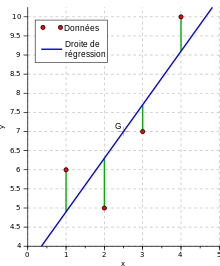
\includegraphics[scale = 0.5]{images/regression_lineaire}
% 	\caption{Graphique d'une régression linéaire classique}
% 	\label{fig:regression_lineaire}
% \end{figure}
%  
% les valeurs Y représente les résultats correspondant aux données de X et $\beta$ Les poids qui permettent de minimiser l'erreur de l'estimation, c'est à dire faire en sorte que la droite passe au plus prés possible de tous les points. 
% La formule de la régression linéaire est la suivante (à 1 dimension): 
% \begin{equation}
% Y = X * \beta + \epsilon
% \end{equation}
% $\epsilon$ est ici un nombre infiniment petit qui représente une variation minime sur tout estimateur car l'erreur est humaine et l'apprentissage aussi. 
% Cette formule nous permet facilement d'isoler $\beta$ afin de le calculer. 
% 
% En ce qui nous concerne, Y correspond à une matrice de dimension n ligne et une colonne. X représente une matrice de n ligne et p colonne ainsi $\beta$ représente une matrice à 1 ligne et p colonne. 
% Donc notre régression se calcul non pas sur une dimension mais sur n dimension. La formule devient donc :
% \begin{equation}
% Y = X_{1} * \beta_{1} +X_{2} * \beta_{2} + X_{3} * \beta_{3} + ... + \epsilon
% \end{equation}
% 
% 
% En nous basant sur cette formule, il est facile après d'isoler les $\beta_{i}$ et de les calculés. 

Une fois nos paramètres estimés, il faut que le Y calculé soit entre 0 et 1. Or, les résultats donnés par la régression linéaire sont définis sur l'ensemble des réels. On applique donc une fonction logistique afin de classés les résultats. 
Ce modèle nous assure un bon ratio des résultats d'apprentissage et de test. Ainsi, nous évitons le problème de sur-apprentissage. 
Ce modèle repose sur des "pénalités". Ces pénalités sont ce que l'on peut appeler des contraintes de parcimonies qui consiste à ce que l'algorithme d'apprentissage apprenne en utilisant le moins de variables descriptives possibles. Ces contraintes permettent à l'algorithme d'éviter de rentrer en sur-apprentissage et aussi de mieux classés les voxels afin d'obtenir une meilleure classification.